\qns{Pulsar Dispersion Measure}

\begin{enumerate}

\qitem{}
\work{
	\begin{enumerate}
		\item Find data where, for a given frequency, there is a clear time at which it peaks. The selection criterion was that the difference between the maxima was some percentage of the absolute maximum for that frequency.
		\item Using 
		$$t_1 - t_0 = \frac{e^2}{2\pi m_ec}(DM)\left(\frac{1}{\nu_1^2} - \frac{1}{\nu_0^2}\right)$$
		estimate the dispersion measure between each pairing of ``good'' data points. Depending on the severity of the selection criteria, it's possible to end up with a negative calculated dispersion ratio; increasing the stringency of criteria for what constitutes a clean peak resolves this.
		\item Find the geometric mean of the data.
	\end{enumerate}}
\ans{
	\centering
	DM $\approx 10^{21} \frac{\text{electrons}}{\si{\centi\meter}^2}$}

\qitem{}
\work{
	\begin{itemize}
		\item $n_e \approx 0.03\frac{\text{electrons}}{\si{\centi\meter^3}}$
	\end{itemize}
	$$\text{DM} = \int_0^d n_e d\ell \approx n_e d$$}
\ans{
	\centering
	$d \approx 10,000$ pc---roughly the distance to the center of the Milky Way.}

\qitem{}
\work{
	$$\nu_p = \frac{1}{2\pi}\sqrt{\frac{4\pi n_e e^2}{m_e}}$$}
\ans{
	\centering
	$\nu_p \approx 1.5\si{\kilo\hertz}$---quite a lot lower than the observation frequency.}

\qitem{}
\work{
	\begin{align*}
		\sigma_\text{Thomson} &= \frac{8\pi}{3}\left(\frac{e^2}{m_ec^2}\right)^2\\
		\tau_\text{Thomson} &= n_e \sigma_\text{Thomson} d
	\end{align*}}
\ans{
	\centering
	$\tau_\text{Thomson} \approx 7(10^{-4}) \ll 1$ so Thomson scattering isn't significant}

\end{enumerate}

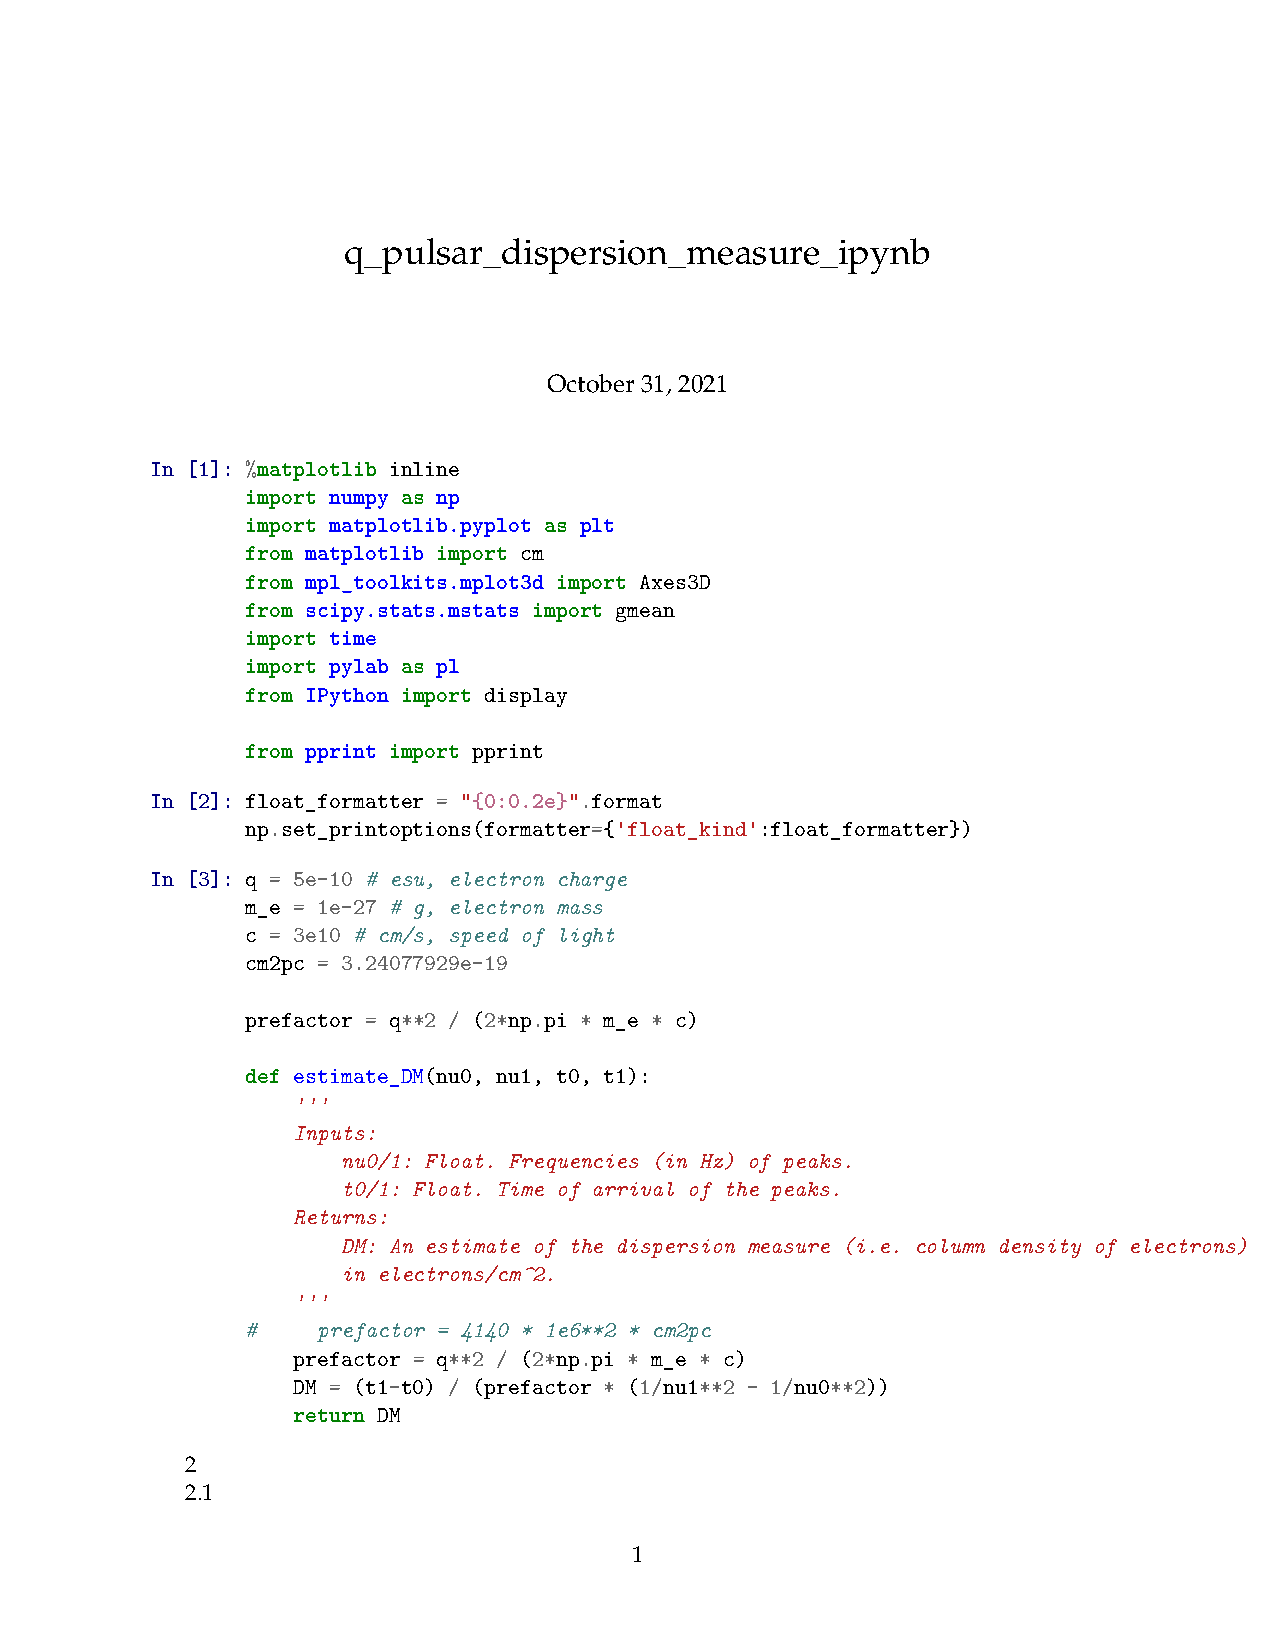
\includepdf[pages=-,pagecommand={},width=\textwidth]{./questions/q_pulsar_dispersion_measure_ipynb.pdf}